\chapter{Análisis de estabilidad}



\section{Criterio de estabilidad de Nyquist}

El criterio de estabilidad de Nyquist nos permite determinar la estabilidad del sistema 
a lazo cerrado analizando el sistema de lazo abierto. 


Si retroalimentos de forma negativa una función de transferencia $G(z)$ con $P_0$ número de polos fuera del círculo unitario,
y $P_c$ del lazo cerrado fuera del circulo unitario esta dado por la ecuación: 

\begin{equation}
    P_c = N + P_0
\end{equation}

Donde $N$ es el número de revoluciones en el sentido agujas del reloj alrededor del punto $-1$ de la grafica $G(z)$, grafico en forma polar, 
cuando "$z$" recorre la trayectoria cerrada que se muestra en la Figura \ref{fig:nyquist}. 

\begin{figure}
    \centering
    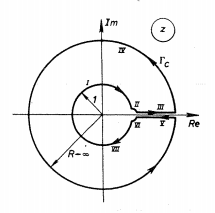
\includegraphics[width=.5\textwidth]{img/nyquist.png}
    \caption{Curva de Nyquist.}
    \label{fig:nyquist}
\end{figure}

\section{Controlabilidad}

Considerando la dinamica del sistema: 

\begin{equation}
    X(n) = \Phi^n X(0) + W_c U
\end{equation}

donde $U=\begin{bmatrix}
    u^T(n-1) & \cdots & u^T(0) 
\end{bmatrix}^T$

El sistema de la ecuación \ref{eq:sis} es controlable COMPLETO si es posible encontrar 
una secuencia de control tal que pueda alcanzarse un estado deseado desde cualquier otro estado. 

El sistema es controlable al ORIGEN, si es posible encontrar una secuencia de control tal que 
el origen se pueda alcanzar desde cualquier estado. 

El sistema es controlable completo si la matriz $W_c$ tiene rango $n$. 

\begin{equation}
    W_c = 
    \begin{bmatrix}
        \Gamma & \Phi \Gamma & \cdots & \Phi^{n-1}\Gamma
    \end{bmatrix}
\end{equation}

Si $\Phi$ es inversible, entonces la controlabilidad al origen implica controlabilidad 
completa. 

\section{Observabilidad}

La observabilidad implica poder medir los estados del sistema, en caso de que
los estados no sean observables y se desee implimentar un control por retroalimentación de
estados es necesario incluir un observador al sistema de lazo cerrado. 

El sistema es observable si y solo si la matriz $W_o$ es de randgo $n$.

\section{Control en espacio de estados}

Sea el sistema de la ecuación \ref{eq:sis}, el controlador será de la forma: 

\begin{equation}
    u(k) = -LX(k)
\end{equation}

La ecuación de lazo cerrado: 

\begin{equation}
    qX(k) = (\Phi - \Gamma L)X(k)
\end{equation}

Es posible diseñar una matriz de ganancia $L$ tal que los autovalos de $\Phi_{lc}$
esten ubicados en cualquier lugar. Para ello, es posible utilzar el teorema de Ackermann, 
donde si $\Phi_{lc}$ tiene ecuación característica arbitraria $P_d(z)$ y 
el sistema es controlable, entonces: 

\begin{equation}
    L = \begin{bmatrix}
        0 & \cdots & 0 & 1
    \end{bmatrix}
    W^{-1}_c P_d(\Phi)
\end{equation}

\section{Deadbeat}

Un sistema de tiempo finito discreto que tiene una respuesta al impulso finita (FIR), 
necesariamente tiene todos sus polos en el origen. Por lo tanto la determinación del 
del controlador queda de la forma: 

\begin{equation}
    L = \begin{bmatrix}
        0 & \cdots & 0 & 1
    \end{bmatrix}
    W^{-1}_c \Phi^n
\end{equation}

\section{Observadores}

En general no todos los estados son medibles, por lo tanto es necesario 
estimar los estados, para ello necesitamos que el sistema sea observable.

\subsection{Cálculo directo de las variables de estado}

El calculo directo posee la ventaja de ser un método rapido desde el punto de vista 
que no incluye una sistema dinamico, como si sucede en los otros métodos. 

\begin{equation}
    \hat{x}(k) = \Phi^{n-1} W^{-1}_o 
    \begin{bmatrix}
        y(k-n+1) \\ 
        y(k-n+2) \\ 
        \vdots \\ 
        y(k)
    \end{bmatrix} + 
    \Psi 
    \begin{bmatrix}
        u(k-n+1) \\ 
        u(k-n+2) \\ 
        \vdots \\ 
        u(k-1)
    \end{bmatrix}
\end{equation}

Donde: 

\begin{equation}
    \Psi = \begin{bmatrix}
        \Phi^{n-2} \Gamma & 
        \Phi^{n-3} \Gamma & 
        \cdots & 
        \Gamma
    \end{bmatrix} - 
    \Phi^{n-1}W^{n-1}_o\Omega
\end{equation}

\begin{equation}
    \Omega = \begin{bmatrix}
        0 & 0 & \cdots & 0 \\ 
        C\Gamma & 0 & \cdots & 0 \\ 
        C\Phi\Gamma & C\Gamma & \cdots & 0 \\ 
        \vdots & \vdots & \ddots & 0 \\ 
        C\Phi^{n-2}\Gamma & C\Phi^{n-2}\Gamma & \cdots & C\Gamma 
    \end{bmatrix}
\end{equation}

\subsection{Reconstrucción mediante un sistema dinámico}

Es posible estimar los estados del sistema utilizando una estimación de la salida, 
similar a la estimación del error, por lo tanto: 

\begin{equation}
    \label{eq:din}
    \hat{x}(k+1|k) = \Phi \hat{x}(k|k-1) + \Gamma u(k) + K[y(k) - C \hat{x}(k|k-1)]
\end{equation}

Donde $K$ debe ser elegida de forma adecuada. 

Si planteamos el error de reconstrucción, obtenemos que: 

\begin{equation}
    \tilde{x}(k+1) = x(k+1) - \hat{x}(k+1|k) 
\end{equation}

Remplazando por las expresiones de las ecuaciones \ref{eq:sis} y \ref{eq:din}

\begin{equation}
    \siseq{
        \tilde{x}(k+1) = \Phi x(k) + \Gamma u(k) - \left\{ 
        \Phi \hat{x}(k|k-1) + \Gamma u(k) + K[y(k) - C \hat{x}(k|k-1)]
    \right \} \\ 
        \tilde{x}(k+1) = \Phi x(k) - \Phi \hat{x}(k|k-1) - K[y(k) - C \hat{x}(k|k-1)] \\ 
        \tilde{x}(k+1) = [\Phi - KC] \underbrace{(x(k) - \hat{x}(k|k-1))}_{\tilde{x}(k)} \\ 
        \tilde{x}(k+1) = [\Phi - KC] \tilde{x}(k)
    }
\end{equation}

Es posible utilizar el teorema de Ackermann, para ello plantemoas que $\tilde{L}=K^T$, $\tilde{W_c}=W_o^T$ y 
$\tilde{\Phi}=\Phi^T$, Por lo tanto: 

\begin{equation}
    K = P_d(\Phi)W_o^{-1}
    \begin{bmatrix}
        0 & 0 & \cdots & 1
    \end{bmatrix}^T
\end{equation}

Si bien el sistema anterior es bueno, es posible utilizar la información actual, por lo tanto: 

\begin{equation}
    \hat{x}(k|k) = \Phi \hat{x}(k-1|k-1) + \Gamma u(k-1) + k[y(k) - C(\Phi \hat{x}(k-1|k-1) + \Gamma u(k-1))]
\end{equation}

Despejando la dinamica del sistema queda: 

\begin{equation}
    \hat{x}(k|k) = [I-KC]\Phi \hat{x}(k-1|k-1) + \Gamma u(k-1) +  Ky(k)
\end{equation}

Cuyo error de reconstrucción esta dado por: 

\begin{equation}
    \tilde{x}(k+1) = (I-KC)\Phi\tilde{x}(k)
\end{equation}

Este observador permite seleccionar $K$ de tal manera de anular 
Distintas filas, lo que se asocia a un estado estimado sin error.
Para estimar $p$ estados sin error en un sistema de $m$, 
es necesario que al menos $p$ salidas seas LI. ($p<m$)
El resto de valores de $K$ se deben elegir para que los polos del sistema 
queden en la zona de interes.

